%!TEX root = ../paper.tex
\subsection{Overview}
The dynamical model given in terms of a system of differential equations for any network can be represented in terms of an interaction graph (\ref{fig:biomodelexamples} top row). These interaction graphs can be viewed as deriving from the combination of system modules that accept a given pattern of inputs and produce a given pattern of outputs (\reffigexamplesystemmodules). Symmetries are characterized by the ability to interchange these modules or their connectivity without changing some property of the system.

The network architecture can be represented in terms of an adjacency matrix and further abstracted by mapping the interaction graph to the network of strongly connected components (SCCs, see \refsupp{}) (\reffigscc). This map from the interaction graph of a biological network, referred to as $\hier$, has a collection of symmetries shown in \reffighiertransformations. These three symmetries represent transformations that can be performed on the interaction graph that do not change the network of SCCs to which it is associated \reffigscc. Two of these three are also symmetries with respect to dynamical robustness. \ref{fig:robustnesssymmetries} shows an example of these symmetries applied to a specific interaction graph.

We have derived an analytical expression for dynamical robustness, $R_{tot}$, of a biological network in terms of its interaction graph as a weighted average of the robustness of the SCCs, $R_i$, the corresponding number of links within each SCC, $d_i$, and the number of links between the SCCs, $l$. This expression is fully developed in \ref{eq:sccrobustness}, but can be schematized as in \ref{eq:robschematic} (see \reffigscc$\,$ for examples demonstrating this expression)
\begin{equation}\label{eq:robschematic}
R_{tot} = \frac{l+d_1 R_1 + d_2 R_2 + \cdots}{l+d_1 + d_2 + \cdots}.
\end{equation}
Examining this expression noting that $R_i$ are all strictly less than one proves that networks maximizing $l$, will also maximize $R_{tot}$.
This implies that the interaction graphs for systems that are the most robust will maximize the number of links between SCCs as well as the overall number of SCCs with respect to a particular system size. This analytical result predicts that any biological network whose associated dynamical system has the interaction graph \reffigscc $\,$ top will be more robust than those associated to any of the other interaction graphs in \reffigscc. Because this result is purely topological in nature, it does not depend at all upon any particular details such as the probability distribution from which the component interaction strengths are sampled or the size of the system. The result that dynamical robustness is correlated with network hierarchy therefore applies to an even broader class of dynamical systems than the particular random ensembles we have studied directly.

To test this prediction, we computed the probability distribution of stability and dynamical robustness relative to biological network architecture for ensembles of systems having two or three interacting components (see \ref{tab:structstabmat} and \ref{tab:structstabmat3}). For all of these, we found that robustness is correlated with connectivity, but that the most robust systems have intermediate connectivity for a given network size (\reffigrobustconnect). Accounting for the number of cycles in a network architecture reveals a strong correlation between robustness and connectivity that was hidden when networks with any number of cycles were considered together (\reffigconnectcycle3D3x3). While the most hierarchical network architecture will always lack cycles altogether, cycle number alone is clearly insufficient to account for robustness as the members of each class span nearly the entire range of possible robustness values. Consistent with our analysis of the symmetries of robustness, we found that the most hierarchical network architecture is the most robust (\reffigrobusthierarchy). Moreover, if we consider hierarchy partitioned by connectivity, we find that there is a monotonic increase in robustness following any line of increasing hierarchy in \reffigconnectdist3D3x3.

\subsection{Dynamical systems on biological networks}
In the construction of a class of potential models for biological systems at any level of the biological hierarchy from metabolic to ecosystem-level networks, it is common to first attempt to define a collection of observable phenomena of interest and determine a domain (such as binary numbers, integers, or real numbers) in which each observable can be quantified. Next, it is necessary to establish the interdependencies among system components. The specific manner in which the components depend upon one another must be clarified, which is often done by determining a particular system of mathematical functions that represents a hypothesis about how the quantified observables evolve in time. To the degree to which there is uncertainty about the interactions among system components, parameters are introduced to broaden the class of models under consideration. Finally, whatever model class remains may be compared to empirical observations to determine how capable the model is of representing the phenomena of interest.

For the case of continuous deterministic observables, the above process can be made more precise by associating a manifold $M_i$ to each observable, a directed graph, $G$, to the interdependencies, and a vector field $V$ over the space determined by taking the product of the manifolds associated to the collection of observables, satisfying these interdependencies for each observable  \cite{Deville}. For example, if we have two observables $\{x_1,x_2\}$ where the domains in which they are quantified are given by manifolds $\{M_1,M_2\}$ such that $x_1 \in M_1 \equiv \mathbb{R}^1$ and $x_2 \in M_2 \equiv \mathbb{R}^1$, a directed graph $G_X$ describing the dependencies between these observables and vector field $V$ with components $\{F_1,F_2\}$ defined on $M_1 \otimes M_2 \equiv \mathbb{R}^2$ satisfying the dependencies determined by $G_X$. If the system under consideration has the graph given in \reffigexamplesystemmodules$\,$
% \begin{center}
% %!TEX root = ../paper.tex
\begin{tikzpicture}[
every state/.style={draw=red!50,very thick,fill=red!20}]
\begin{dot2tex}[styleonly,codeonly,neato,mathmode]
digraph G {
d2ttikzedgelabels = true;
node [style="state"];
edge [lblstyle="auto",topath="bend left",style="line width=1.5pt"];
x_1 -> x_2;
x_2 -> x_1;
x_2 -> x_2 [topath="loop above"];
}
\end{dot2tex}
\end{tikzpicture}

% \end{center}
with adjacency matrix
$$
\adj(G_X) = \begin{pmatrix}
0 & 1 \\
1 & 1
\end{pmatrix}
$$
having connectivity $\connectivity$ equal to the number of edges of the graph, in this case $\connectivity = 3$. For a general system the directed graph $G_X$ that describes the manner in which each of the variables depends upon one another is given by the adjacency matrix $\adj(G_X)$ where
 \begin{displaymath}
   \adj(G_X)_{ij} = \left\{
     \begin{array}{ll}
       1, & F_i \hbox{ depends on } x_j\\
       0, & F_i \hbox{ does not depend on } x_j
     \end{array}.
   \right.
\end{displaymath} For the system $X = \{G_X, M_X, F_X\}$, where $M_X \equiv \{M_1,M_2\}$ and $F_X \equiv \{F_1,F_2\}$ such that $F_1$ is a function of $x_2$ alone and $F_2$ is a function of both $x_1$ and $x_2$ yielding the flow equations
\begin{align*}
\frac{dx_1}{dt} & = F_1(x_2),\\
\frac{dx_2}{dt} & = F_2(x_1,x_2).
\end{align*}

In the more general case of a system with $n$ components we would have an $n$-dimensional vector of observables
$$
x(t) = (x_1(t), \ldots x_n(t)) = \vec{x}(t)
$$
whose components are solutions to the arbitrary first order system
$$
\frac{dx_i(t)}{dt} = F_i(\vec{x}(t)), \; (i=1,\ldots,n)
$$
where $F_i$ represent, potentially nonlinear, functions of the given vector of state variables.

In order to accommodate the possibility of uncertainty in our
modeling, we will generalize our notion of a system on a network to
that of a system with random parameters.  Again, this will involve
three steps. First, we provide a measure space $S$
which represents the values over which our parameters can vary. Next,
instead of a single vector field, we consider a family of vector
fields parameterized by this space.  As before, for
each point $p \in S$, the vector field $V(p)$ must be consistent with
the system graph. Finally, we select a probability measure $\mu$ which represents our understanding of which values of the parameters
are likely. In accord with Bayesian statistics, we might revise this
distribution as data comes in or use it to estimate parameters and error
bars from experimental results.

Having done this, we are now in a position to do a probabilistic analysis
of our system and its properties.  Given some quantity $q$ characterizing
our system, this quantity becomes a random variable which may be discrete or
continuous depending on the quantity under consideration.  For example, if
the quantity is the time it takes for a particle to travel between two points,
we have a real-valued random variable; if the quantity is the number of fixed
points, we have an integer-valued random variable; and if the quantity is
whether or not the system posesses a limit cycle, we have a binary random
variable.

A quality which is of interest to us is robustness whose evaluation requires the determination of whether or not a given dynamical system that is determined to be stable remains stable under a perturbation to one or more of its defining parameters \footnote{We mean to refer to perturbations to the structure of the system itself as determined by the strengths of the couplings between the components as determined by the parameters and not only to perturbations of the state vector at a given point in time. For example, when the network of components and interactions corresponds to a gene-regulatory network, then mutation is one mechanism by which such perturbations may arise}.  We will quantify this as the probability that, if some property holds for a set of parameters, it will continue to hold if we make a random perturbation about those parameter values. To do so, we will introduce, in addition to the probability distribution $\mu$ described above, a family of probability distributions $\mu'$ such that $\mu'(x,y)$ encodes the conditional probability that a system with a parameter value $x$ will have its parameter values changed to $y$ under a perturbation.  For our biological models, we will be interested in large perturbations rather than the small or infinitesimal perturbations usually considered in the theory of dynamical systems.  Then, given a binary random variable $q$, we define its robustness as the following conditional probability where $\mathbf{1}_q(x)$ is the standard indicator function equal to $1$ when $x$ satisfies $q$ and $0$ otherwise:
\begin{align}\label{eq:robustness}
  R (q,\mu') =
  \frac{\int_S d\mu(x) \int_S d\mu'(x,y) \mathbf{1}_q(x) \mathbf{1}_q(y)}
  {\int_S d\mu(x) \mathbf{1}_q(x)}
\end{align}

\subsection{Stability analysis of biological networks}
The class of dynamical quantities on which we shall focus in this
investigation involve stability of equilibria.  Suppose that $\vec x$
is a point on our phase space which depends upon the parameters.  Then
we may take $q$ to be a binary random variable which describes whether
or not $\vec x$ is a fixed point of the system (i.e. $q$ is true if and only if
$F_i(\vec{x})=0$ for all $i$) and perform a probabilistic analysis
of the sort discussed above.

Furthermore, if it turns out that $\vec x$ is indeed a fixed point, we
may proceed to ask whether it is a dynamically stable fixed point.
Intuitively, dynamic stability means that, if one chooses the initial
conditions sufficiently close to the fixeed point, the solution will
stay close to the fixed point.  Physically, this is important because,
if a fixed point ${\vec x}^0$ is unstable, we have zero probability of
observing the solution ${\vec x}(t) = {\vec x}^0$.

To determine stability, we linearize the equations of motion about the
fixed point $\vec{x}^0$:
\begin{equation}\label{eq:lineardynsys}
\frac{d\vec{y}(t)}{dt} = A \vec{y}(t),
\end{equation}
where $\vec{y} = \vec{x} - \vec{x}^0$ and the $n \times n$-matrix $A$ has components
$$
a_{ij} = \left. \frac{\partial F_i}{\partial x_j} \right|_{\vec{x} = \vec{x}^0}.
$$
To each dynamical system having Jacobian matrix $A$ at some fixed point $\vec{x}^0$ we can associate a directed graph $G_A$ given by an adjacency matrix $\adj(G_A)$ where
 \begin{displaymath}
   \adj(G_A)_{ij} = \left\{
     \begin{array}{lr}
       1, & a_{ij} \neq 0\\
       0, & a_{ij} = 0
     \end{array}
   \right.
\end{displaymath}
The graphs $G_X$ and $G_A$ are equivalent because the condition $F_i$ independent of $x_j$ definitive of $\adj(G_X)$ corresponds precisely to $\frac{\partial F_i}{\partial x_j}=0$.

The spectral abscissa of the matrix $A$ is defined as
$$
\eta(A) = \max_i \{\Re(\lambda_i)\}
$$
where $\lambda_i$ are the eigenvalues of $A$. The system defined by $F_i$ and $\vec{x}^0$ is dynamically stable if the spectral abscissa of $A$ is less than zero, equivalently, $\eta(A) < 0$. This is because the general solution to \ref{eq:lineardynsys} is
$$
y_i(t) = \sum_j b_{ij} e^{\lambda_j t}, \; (i=1,\ldots,n)
$$
for some matrix $B=(b_{ij})$ and thus all $\vec{y} = \vec{x} - \vec{x}^0$ decay to zero when all $\lambda_i < 0$. This criterion can be checked equivalently in terms of conditions on the coefficients of the characteristic polynomials $\chi(A)$ associated to the systems described by matrices $A$ \cite{Gantmacher1959}.

Even though the determination of stability only requires examining
linearized equations of motion, it is worth noting that knowing the
stability of a fixed point can yield information about the non-linear
dynamics of a system.  For instance, in two dimensions,
Poincare-Bendixson theory implies that every limit cycle must encircle
at least one fixed point \cite{Davis1962}.  Furthermore, in the case where the cycle contains a single fixed point (such as in the Lotka-Volterra model of
conflicting populations), the stability of the fixed point will determine whether the limit cycle is attractive or repulsive.

%% To determine whether a randomly selected dynamical system evaluated at
%% a random critical point, given by a matrix such as $A$, is stable, it
%% is sufficient to check the above condition. Integrating over the
%% region of the parameter space defining $A$ enables the determination
%% of the probability of stability to perturbations in state $\vec{x}$
%% over an ensemble of dynamical systems.

% Another form of stability, referred to as structural
% stability \cite{Smale1967}, requires the determination of whether or
% not a given dynamical system that is determined to be stable remains
% stable under a perturbation to one of its defining parameters. This
% can be formalized as the conditional probability distribution
% $$
% P(A' \, \textrm{stable}\, \big| \, A \, \textrm{stable})
% $$
% where $A'$ represents a matrix derived from some perturbation
% applied to the matrix $A$ given above. In the simple case where
% $A \in \mathbb{R}^{n \times n}$ the perturbation which involves
% sampling uniformly over the $a_{ij}$ defining $A$ the value of a
% particular $a_{ij}$ from a given probability distribution.

Suppose that our Jacobian $A$ is an $n \times n$ matrix with real coefficients, connectivity $\connectivity$, and denote the proposition ``$A$ is stable'' as $\mathrm{stab}(A)$.  Then we may compute the robustness of this proposition using \ref{eq:robustness} once we have specified the probability densities $\mu$ and $\mu'$.  In general, these will depend upon the parameters of the non-linear system.  For the purpose of the current investigation, we shall make the ansatz that these are such that the distribution of entries of $A$ is (at least approximately) the uniform distribution $\mathcal{U}(-1,1)$ on the $\connectivity$-dimensional hypercube, $H^\connectivity$, of edge length $r=2$, centered about the origin. To model the perturbations, we resample the elements $k_1, k_2, \ldots k_m$ of this matrix from the same uniform distribution yielding
\begin{widetext}
$$
\mu_{k_1,\ldots,k_m}(x,y) = \prod_{y \notin \{x_1, \ldots, x_m\} } \delta(x_j-y_j) \prod_{y \notin \{x_1,\cdots,x_m\}} \mathbf{1}_{[-1,1]} (y_j) \mathbf{1}_{[-1,1]} (x_j)
$$
\end{widetext}
Under these assumptions, the expression for robustness becomes a special case of \ref{eq:robustness}:
\begin{widetext}
\begin{equation}\label{eq:condprobgen}
 R (\mathrm{stab}, \mu'_{k_1, \ldots, k_m}) =
  \frac{\int_{H^\connectivity} dx_1 \cdots dx_d \int_{H^m} {dx'}_{k_1} \cdots {dx'}_{k_m}\,
    \mathbf{1}_{stab} \mathbf{1}_{stab'}}
  {\int_{H^\connectivity} dx_1 \cdots dx_d  \, \mathbf{1}_{stab}(x_1 \cdots x_d)},
\end{equation}
\end{widetext}
where we use the abbreviations
\begin{align*}
\mathbf{1}_{stab} &= \mathbf{1}_{stab}(x_1 \cdots x_{k_1} \cdots x_{k_m} \cdots x_\connectivity), \\
\mathbf{1}_{stab'} &= \mathbf{1}_{stab'}(x_1 \cdots {x'}_{k_1} \cdots {x'}_{k_m}  \cdots x_d),
\end{align*}
i.e. $\mathbf{1}_{stab'}$ corresponds to replacing $x_{k_1}, \ldots x_{k_m}$ with their primed counterparts.

While one can resample a fixed subset of the links, more typically we will be randomly selecting which links to resample with a uniform distribution on the links.  The result of this operation corresponds to averaging our quantity over subsets of links:
\begin{widetext}
\begin{equation}\label{eq:robavgoverlinks}
\langle R (\hbox{stab}, \mu') \rangle_m =
\frac{1}{\binom{\connectivity}{m}}
\sum_{\{k_1, k_2, \ldots k_m\} \subset \{1, 2,, \ldots \connectivity\}}
R (\hbox{stab}, \mu'_{k_1, \ldots, k_m})
\end{equation}
\end{widetext}
We are fundamentally interested in the relationship between \ref{eq:condprobgen} and \ref{eq:robavgoverlinks} and topological properties of systems that derive from their associated graphs. In order to investigate this further, we must characterize properties of system graphs in order to evaluate correlations of those properties with dynamical robustness.

\subsection{Network hierarchy and strongly connected components}

Dynamical networks of the kind described above can be viewed at the level of their interdependency graphs as being composed of more fundamental interacting subsystems \reffigexamplesystemmodules. One such kind of system composition and decomposition is given by the notion of open systems, which are distinguished by having some of the variables specified as control variables whose values are given as autonomous functions of time rather than determined by the dynamics via intrinsic interactions \cite{Vagner2014}.  Given several such open systems, we may combine them to produce a larger system by setting the control variables of a subsystem equal to the dynamical variables of another system.  Taking this notion to its logical extreme, one can dissect a system into a collection of one open system for each dynamical variable.  However, this decomposition is trivial since it is equivalent to the underlying system graph and what we instead want is an intermediate decomposition into relatively self-contained modules.  One method of accomplishing this based upon the topology of the system graph is the decomposition into strongly connected components.

\begin{figure*}[!ht]
\centering
\noindent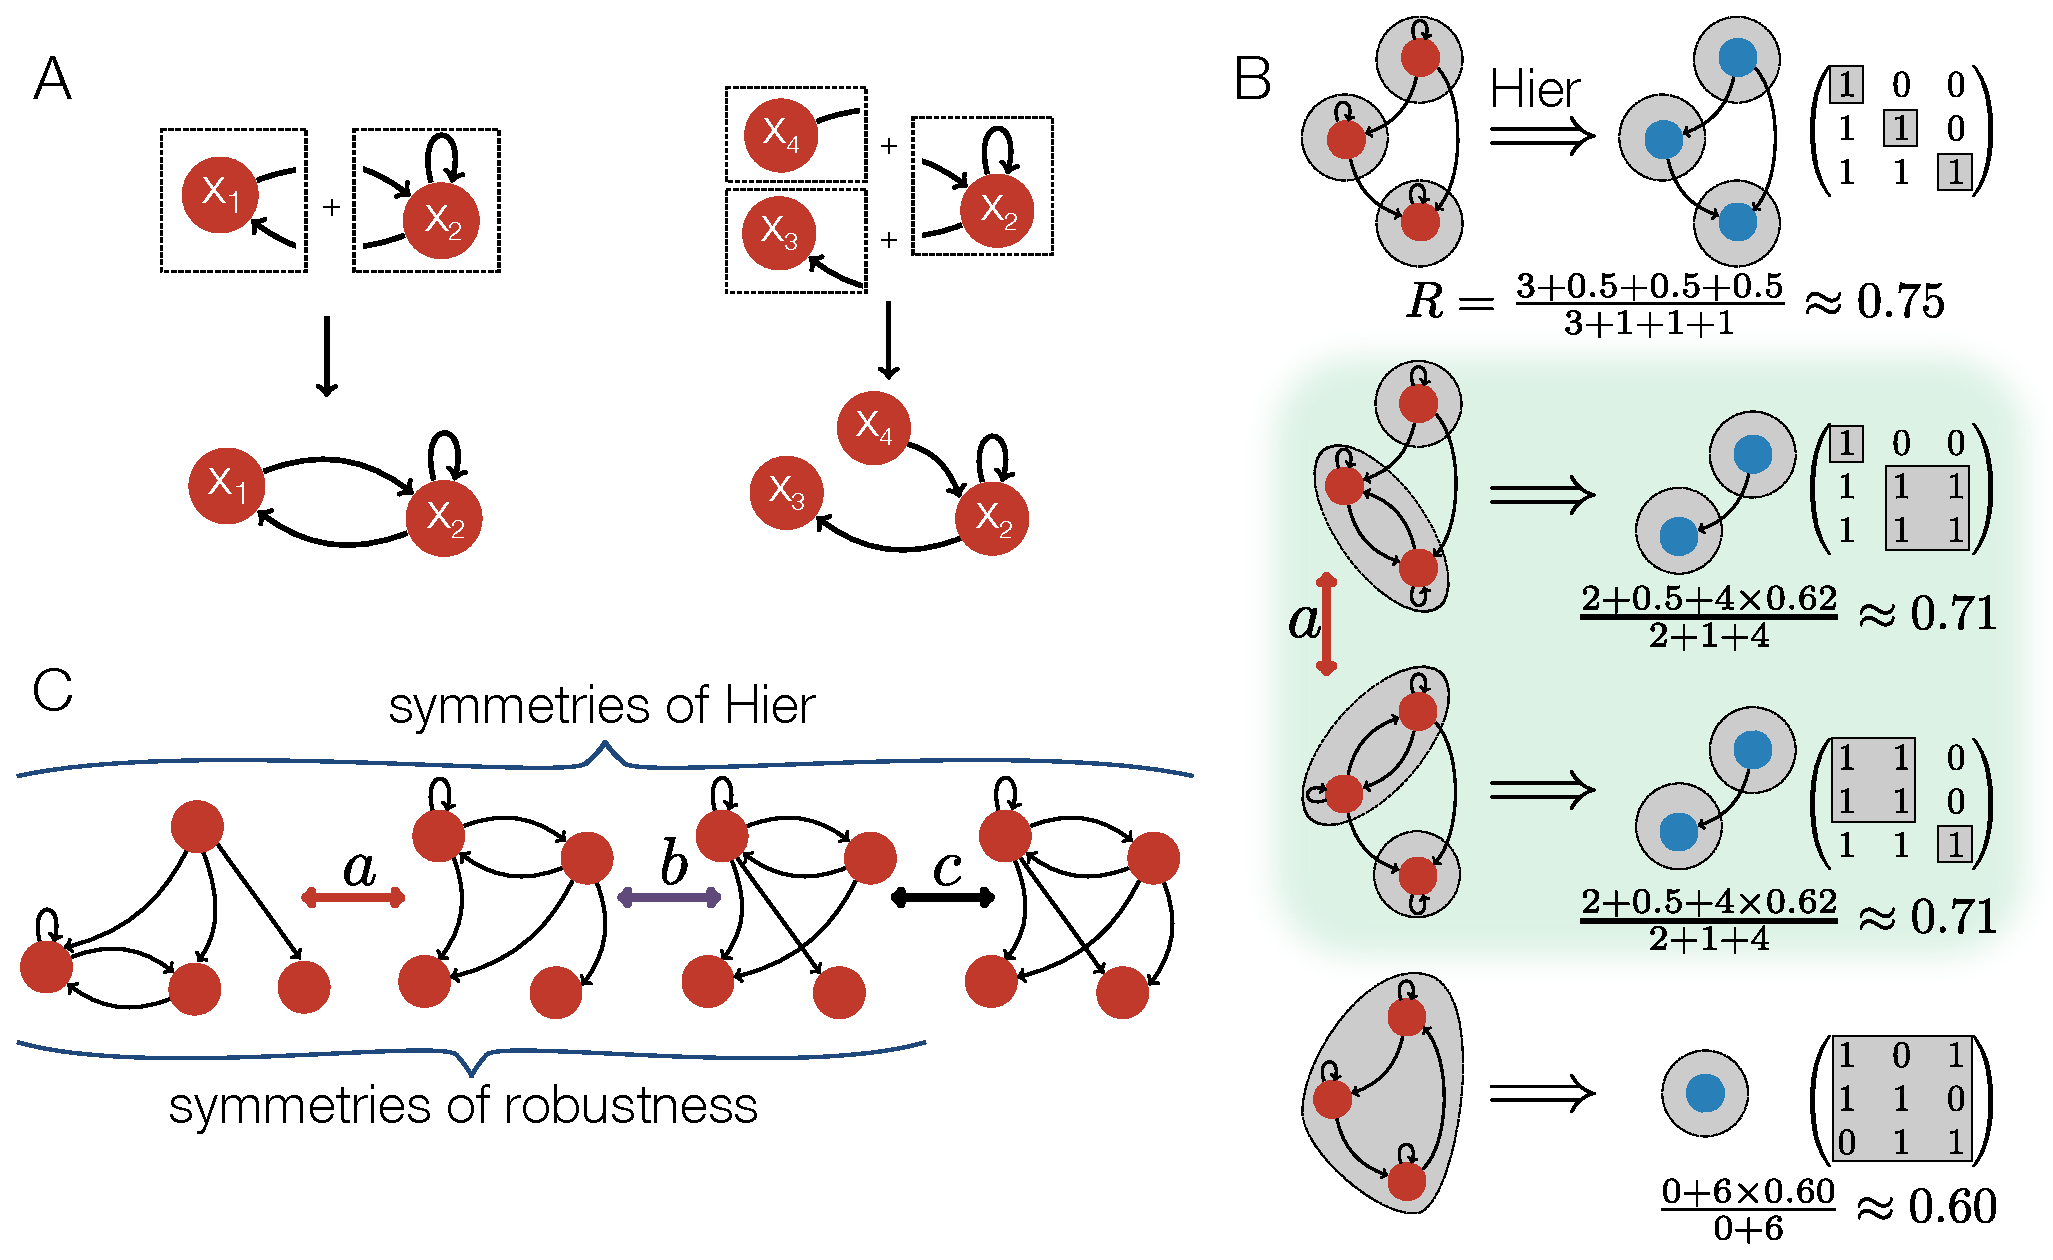
\includegraphics[width=0.8\textwidth]{fig/modsccsym.pdf}
\caption{{\bf Open systems, strongly connected components and symmetries of robustness.} (A) Example of the combination of open system modules to construct closed systems. (B) SCCs highlighted in gray for each of the four graphs representing the interdependencies relevant to four different three variable systems. The most hierarchical network, top panel, is the one that maximizes the number of SCCs and the number of links between them. We therefore define hierarchy as $max(\hbox{ED}) - \hbox{ED}$ where ED is the edit distance representing the number of link addition/deletion operations necessary to transform a given graph into the most hierarchical one. The two panels in the middle represent examples of hierarchical modular systems that posess both modularity (i.e. SCCs with more than one variable) and hierarchy. (C) Symmetries of the $\hier$ transformation between graphs and SCCs. The transformation $a$ represents an interchange of SCCs, $b$ moving a link between nodes in a component and $c$ adding a link. All three transformations represent symmetries of the $\hier$ transformation from graphs to SCCs while only $a$ and $b$ are symmetries of robustness.}
\label{fig:modsccsym}
\end{figure*}

A strongly connected component (SCC) of a graph is a maximal subset of vertices where each vertex within the subset can be reached from any other \cite{Cormen2009}. The strongly connected components of some examples of three variable systems are outlined in \reffigscc$\,$ along with their adjacency matrices and hierarchy diagrams (to be defined below).
The decomposition of a digraph into strongly connected components corresponds to a block triangular decomposition of its adjacency matrix.  Say that the graph $G$ has strongly connected components $C_1, C_2, \ldots C_n$, which have been labelled in such a way that there are no links from vertices in component $C_i$ to component $C_j$ when $i < j$.  Label the vertices in such a way that $v_1, \ldots, v_{n_1}$ belong to $C_1$, $v_{n_1 + 1}, \ldots, v_{n_2}$ belong to $C_2$, etc.  Then, if we choose basis vectors corresponding to this labelling of the vertices, we will have $a_{ij} = 0$ whenever $i$ and $j$ correspond to different components and $i > j$.  This condition is equivalent to stating that the matrix is block triangular with blocks of size $n_1, n_2, \ldots$.

Corresponding to this decomposition we can construct a directed acyclic graph $\hier (G)$ or the condensed graph \cite{Corominas-Murtra2013}.  Each node of $\hier (G)$ corresponds to a strongly connected component of $G$. There is an edge from the node corresponding to component $C$ to the node corresponding to component $C'$ if and only if there exists a link from some vertex in $C$ to some vertex in $C'$ in $G$.  Because of the maximality of strongly connected components, $\hier (G)$ is acyclic.

One can also perform this construction in the opposite direction.  Start with a directed acyclic graph $A$.  To each node $n$ of $A$ associate
a strongly connected graph $C_n$.  To each link $(i,j)$ of $A$ associate a non-empty subset of $\Vertex(C_i) \times \Vertex(C_j)$.  The result will be a graph $G$ such that $\hier(G) = A$ and furthermore, every graph $G$ such that $\hier(G) = A$ can be obtained in this manner.

This map $\hier$ is many-to-one and so there is a large class of
operations which leaves $\hier(G)$ invariant for a given graph $G$.
For instance, we may interchange the positions of the strongly
connected components relative to each other \reffighiertransformations$a$.  Leaving the components fixed, we may move links between nodes in a component \reffighiertransformations$b$ or between components, or even add or delete links \reffighiertransformations$c$.  As we shall see later, some of these operations leave invariant key dynamical quantities, in our case dynamical robustness, so we may regard them as a symmetry groupoid of our system with respect to the robustness property.

The relationship between $G$ and $\hier(G)$ for all $G$ with a given number of vertices suggests a heuristic method of quantifying the degree of hierarchy of a given graph and thus of the system structure it represents. The most hierarchical system is considered to be the graph corresponding to the total ordering, which for three nodes is given in \reffigscc (top panel). This graph maximizes the number of links between strongly connected components, which also implies maximizing the number of strongly connected components. The graph edit distance (ED) on a fixed number of vertices from one graph to another is defined as the minimum number of modifications of the first graph in order to transform it into the second \cite{Axenovich2011}. This distance between any given graph and the total ordering thus quantitatively represents how far a graph is from being perfectly hierarchical. In this work we take $max(ED) - ED$ to be the definition of hierarchy, where $max(ED)$ is the maximum edit distance for all graphs with a given number of nodes.

\subsection{Stability and robustness analysis of particular system ensembles}
For systems having two variables, we can analytically compute the probability of stability and robustness from \ref{eq:condprobgen}. For those having three variables, we can estimate these same quantities using Monte Carlo simulations. Systems of larger size can be analyzed using the symmetry properties of robustness extracted from this analysis. For two-variable systems having $2 \times 2$ Jacobian matrices, the aforementioned stability criteria result in the conditions $T < 0$ and $D >
0$ where $T$ and $D$ denote the trace and the determinant. Suppose we have a stable matrix
$$
\begin{bmatrix}
a & b \\
d & c
\end{bmatrix}
$$
where $a + c < 0$ and $ac > bd$.  For the case in which $x_1=a,\,x_2=b,\,x_3=c,\,x_4=d$ we need to compute what corresponds to $R(\mathrm{stab},\mu'_k)$ where $k=1 \ldots 4$. By symmetry, there are two cases to consider; resampling $a$ is equivalent to resampling $c$ and resampling $b$ is equivalent to resampling $d$ so we only need to explicitly compute $ R(\mathrm{stab},\mu'_1)$ and $R(\mathrm{stab},\mu'_2)$. Suppose that we resample $b$ to compute $R(\mathrm{stab},\mu'_2)$.
% \begin{strip}
% \begin{align}\label{eq:condprob}
% P\left(\begin{pmatrix}
% a & b' \\
% d & c
% \end{pmatrix} \textrm{stable } \bigg| \begin{pmatrix}
% a & b \\
% d & c
% \end{pmatrix} \textrm{stable } \right)
% & = \frac{P\left(\begin{pmatrix}
% a & b \\
% d & c
% \end{pmatrix} \textrm{stable and } \begin{pmatrix}
% a & b' \\
% d & c
% \end{pmatrix} \textrm{stable } \right)}{P\left(\begin{pmatrix}
% a & b \\
% d & c
% \end{pmatrix} \textrm{stable } \right)}.
% \end{align}
The denominator of \ref{eq:condprobgen} in this case is given by
\begin{align*}
P\left(\textrm{stab } \left( \begin{bmatrix}
a & b \\
d & c
\end{bmatrix} \right) \right) = \frac{\int_{\genfrac{}{}{0pt}{}{\genfrac{}{}{0pt}{}{ac>bd}{a+c<0}}{H^4}} da\,db\,dc\,dd\,1}{\int_{H^4} da\,db\,dc\,dd\,1}.
\end{align*}
Since the trace does not involve $b$, the $T<0$ condition will be satisfied automatically and we only need to examine the determinant. Thus, we have the inequalities $ac > b'd$ and $-1 < b' < 1$ in addition to the previous constraints leading to an expression for the numerator of \ref{eq:condprobgen}
\begin{widetext}
\begin{align*}
P\left(\textrm{stab} \left( \begin{bmatrix}
a & b \\
d & c
\end{bmatrix} \right) \textrm{ and stab} \left( \begin{bmatrix}
a & b' \\
d & c
\end{bmatrix} \right) \right) = \frac{\int_{{{ac>b'd \atop ac>bd} \atop a+c<0} \atop H^5} da\,db\,dc\,dd\,db'\,1}{\int_{H^5} da\,db\,dc\,dd\,db'\,1}.
\end{align*}
\end{widetext}
The analogous equation for resampling $a$ is
\begin{widetext}
\begin{align*}
P\left(\textrm{stab} \left( \begin{bmatrix}
a & b \\
d & c
\end{bmatrix} \right) \textrm{ and stab} \left( \begin{bmatrix}
a' & b \\
d & c
\end{bmatrix} \right) \right) = \frac{\int_{{{{a'c>bd \atop a' + c < 0} \atop ac>bd} \atop a+c<0} \atop H^5} da\,db\,dc\,dd\,da'\,1}{\int_{H^5} da\,db\,dc\,dd\,da'\,1}.
\end{align*}
\end{widetext}
Using this approach the probability of stability and of robustness for all two variable systems is given in \ref{tab:structstabmat}.

The analogous results for all three variable systems are computed using Monte Carlo integration and shown in \ref{tab:structstabmat3} and \reffigrobustconnect. This process is associated with some error relative to the exact integration described above. In all simulations we use $N~=~10000$ so that the maximum error for $\hat{\theta}~=~0.5$ is $\sigma~=~\sqrt{\mathrm{var}(\theta | \mathcal{D})} \approx 0.005$ (see \emph{Methods}).

It has been stated previously on the basis of simulation that system stability decreases with connectivity as the system size goes to infinity \cite{May1972}. For small system sizes such as the two and three variable systems, studied here the situation is not so clear cut. For two variable systems, system stability is constant across the entire range of connectivities. For three variable systems, the trend shows a minor decrease from connectivity $4$ to $5$ followed by small fluctuations as shown in \ref{fig:apstab3x3}.

The relationship between connectivity and robustness for two variable systems is shown in \ref{tab:structstabmat} and likewise for three variable systems in \ref{tab:structstabmat3} and \reffigrobustconnect. If we average over the different classes of matrices for a given connectivity we see there is a correlation between connectivity and robustness demonstrated by the red dots in \reffigrobustconnect.
% \subsection{Cycle number is inversely correlated with robustness}
\ref{fig:cycle3x3} shows the robustness for all three variable systems as a function of the number of simple cycles (elementary circuits) of length greater than one in the corresponding directed graph \cite{Johnson1975}. There appears to be a weak negative correlation between robustness and the number of simple cycles.

% \subsection{Cycle number and connectivity classify robust systems}
The combination of connectivity and cycle number as shown in \reffigconnectcycle3D3x3 provides a better classification of the dependence of robustness upon network topology. Here the robustness of three variable systems with a given number of cycles, increases monotonically with connectivity. The network with the highest robustness for three variable systems is that of \reffigscc (top panel). This network is the most hierarchical of all three variable systems in the sense that it represents a total ordering of the components of the network and its adjacency matrix also shown in \reffigscc (top panel) has a block triangular structure.

This observation suggested that graph edit distance from \reffigscc (top panel), hierarchy, might provide a better characterization of dynamical robustness. \reffigrobusthierarchy$\,$ shows dynamical robustness as a function of hierarchy. There is a monotonic correlation between the upper bound of robustness and hierarchy. \reffigconnectdist3D3x3$\,$ shows dynamical robustness as a function of both hierarchy and connectivity. The monotonic correlation between hierarchy and robustness is refined by an underlying correlation between robustness and connectivity analogous to that of \reffigconnectcycle3D3x3.

\begin{figure*}[!ht]
\centering
\noindent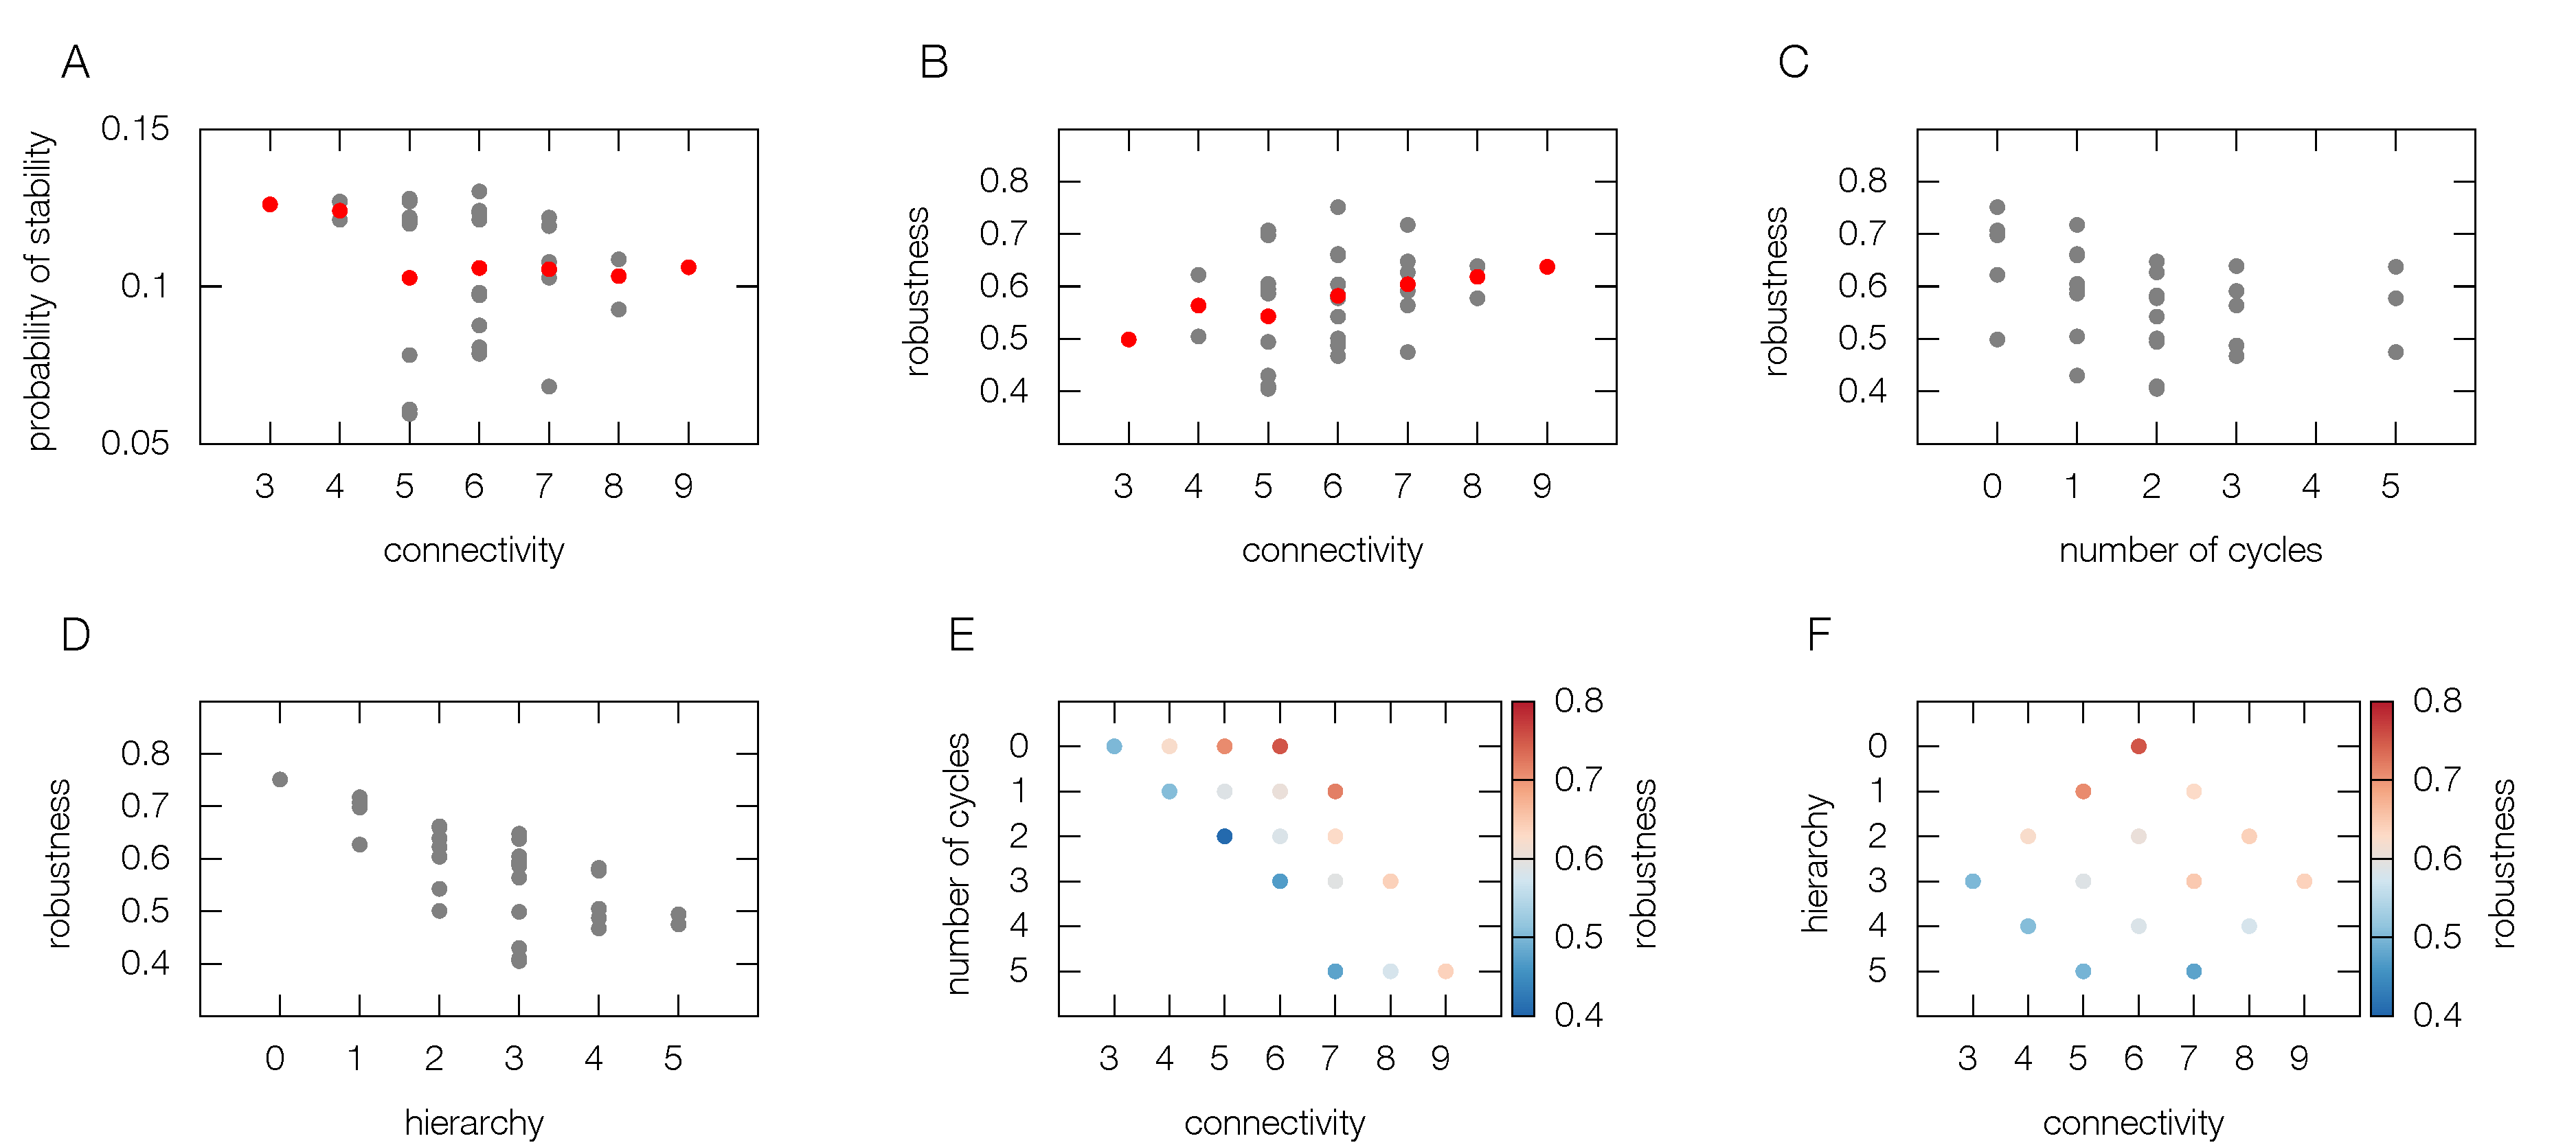
\includegraphics[width=0.8\textwidth]{fig/combinedfigs.pdf}
\caption{{\bf Characterization of stability and robustness according to properties of system structure for three variable systems} (A) Robustness versus connectivity. The red line represents a best fit in the least-squares sense with Pearson product-moment correlation coefficient $r=0.29$. The lowest and highest robustness network architectures are labelled. Other network architectures are shown in \ref{tab:structstabmat3}. (B) Robustness versus hierarchy. Correlation coefficient $r=0.67$. (C) Number of cycles and (D) hierarchy vs connectivity and robustness. The color of each point represents the average robustness of all graphs having the parameters specified on the $x$ and $y$ axes.
}
\label{fig:combined}
\end{figure*}

\subsection{Component decomposition, hierarchy, and the symmetries of robustness}

The fact that the most hierarchical of networks is the most robust in the case of three variable systems can be understood in general as resulting from the previously mentioned symmetry property of network robustness.  By combining our decomposition of the graph with our analysis of the robustness of random ensembles of dynamical systems, we will deduce a general result which relates robustness to hierarchy.

Since the determinant of a triangular matrix equals the product of the determinants of its diagonal blocks, it follows that the characteristic polynomial factors as the product of the charactericstic polynomials of its diagonal blocks.  Hence, a block triangular matrix is stable if and only if its diagonal blocks are stable.  Note that this condition does not depend upon the entries off the diagonal (which correspond to links between strongly connected components) and does not depend upon what order the components appear.

Using these observations, we may express the robustness of a graph in
terms of the robustnesses of its strongly connected components.  If
each component $C_i$ of our graph $G$ has $v_i$ vertices, connectivity
$\connectivity_i$, and there are $\ell_{ij}$ links between components
$i$ and $j$, then there are a total of
$\sum_{i,j \in \hier(G)} \ell_{ij} + \sum_{i=1}^n \connectivity_i$
links in $G$.  If we resample a randomly chosen link in a component
$C_i$, then the probability that the system will remain stable after
resampling is $\langle R(\hbox{stab} (C_i), \mu') \rangle_1$.  If we resample a link
between components $C_i$ and $C_j$, the system will remain stable with
probability 1.  Hence, the probability that the system will remain
stable upon resampling a random link is the weighted average of these
probabilities:
\begin{widetext}
\begin{align}\label{eq:sccrobustness}
\langle R(\hbox{stab} (G), \mu') \rangle_1 =
\frac{\sum\limits_{(i,j) \in \hier(G)} \ell_{ij} +
      \sum\limits_{i=1}^n \connectivity_i \langle R(\textrm{stab}(C_i),\mu') \rangle_1}
     {\sum\limits_{(i,j) \in \hier(G)} \ell_{ij} +
      \sum\limits_{i=1}^n \connectivity_i}.
\end{align}
\end{widetext}
For instance, if our graph is the one in \reffigscc (middle panels), then we have two connected components, one with two nodes, and one with one node.  From \ref{tab:structstabmat}, we know that the graph with two nodes has probability $0.25$ of being stable and robustness $0.62$.  The graph with one node corresponds to a $1 \times 1$ matrix, so we have probability $0.5$ of stability and robustness $0.5$.  Thus, the probability of our 3-node graph being stable is $0.5 \times 0.25 = 0.125$ and its robustness is
\[
\langle R(\textrm{stab}(G),\mu') \rangle_1 = \frac{2 + 0.5 + 4 \times 0.62}{2 + 1 + 4} = 0.714,
\]
which agrees with the value computed in \ref{tab:structstabmat} up to
sampling error.

As can be seen from \ref{eq:sccrobustness}, all that is required to fix robustenss is a set of SCC sizes and the number of links between them. This demonstrates that robustness is symmetric under the transformations shown in \reffighiertransformations $a$ and $b$. Since transformations of the type \reffighiertransformations $c$ change the number of links between connected components, this symmetry of $\hier$ is broken by \ref{eq:sccrobustness}. Nevertheless, a considerable degree of symmetry remains. For example, \ref{fig:robustnesssymmetries} shows the symmetry groupoid of robustness for the case in which we fix connected component sizes $\{2,1,1\}$ with a total of $3$ links between them.

Next, we derive an upper bound on the robustness of any graph
constructed from a given set of connected components.  Since
$\langle R(\textrm{stab}(C_i), \mu') \rangle_1 \le 1$ for all $i$, it follows that increasing $\ell_{ij}$ will
increase $\langle R(\textrm{stab}(G),\mu') \rangle_1$.  Given two connected components $C_i$ and $C_j$ with
$v_i$ and $v_j$ nodes respectively, we have a maximum of $v_i v_j$
links going from $C_i$ to $C_j$.  Hence, $\ell_{ij} \le v_i v_j$, so,
we conclude that
\begin{align}
\langle R(\textrm{stab}(G),\mu') \rangle_1 \le \frac{\sum\limits_{(i,j) \in \hier(G)} v_i v_j +
               \sum\limits_{i=1}^n \connectivity_i \langle R(C_i,\mu') \rangle_1}
              {\sum\limits_{(i,j) \in \hier(G)} v_i v_j +
               \sum\limits_{i=1}^n \connectivity_i},
\end{align}

Since every acyclic digraph can be embedded into a totally ordered
set, we may assume without loss of generality that our components have
been ordered in a way such that, if $(i,j) \in \hier(G)$, then $i <
j$.  Hence, after substituting into our expression and simplifying
using the identity
$$\sum_{i=1}^{n-1}\sum_{j=i+1}^{n}v_i
v_j~=~\frac{1}{2} \left( \sum_{i=1}^{n} v_i \right)^2-\frac{1}{2} \sum_{i=1}^{n}
v_i^2,$$
we arrive at the following upper bound on robustness in terms
of the connected components:
\begin{widetext}
\begin{align} \label{eq:sccmaxrobustness}
R_{\mathrm{max}}(C_1, \ldots C_n) =
\frac{\frac{1}{2} ((\sum_{i=1}^n v_i)^2 - \sum_{i=1}^n v_i^2) +
                    \sum_{i=1}^n \connectivity_i \langle R(\hbox{stab}(C_i),\mu') \rangle_1}
     {\frac{1}{2} ((\sum_{i=1}^n v_i)^2 - \sum_{i=1}^n v_i^2) +
                    \sum_{i=1}^n \connectivity_i}.
\end{align}
\end{widetext}
Furthermore, this bound is attained.  Suppose that $G_{\mathrm{tot}}$
is the graph on $n$ nodes with a link from node $i$ to node $j$
whenever $i < j$.  Then, by the construction described in the previous
section on network hierachy, we have a graph $G_{\mathrm{max}}$ such
that the components of $G_{\mathrm{max}}$ are $C_1, \ldots C_n$ and
$\hier (G_{\mathrm{max}}) = G_{\mathrm{tot}}$.  By our formula,
$\langle R(\hbox{stab} (G_{\mathrm{max}}), \mu') \rangle_1 = R_{\mathrm{max}}(C_1, \ldots C_n)$.

This argument also works when we resample more than one entry,
although the notation becomes more complicated.  Suppose that we
resample $m$ nodes.  Define
\begin{widetext}
\begin{equation*}
M = \left\{(m_0, m_1, \ldots, m_n) \,\bigg|\,
m = \sum_{i=0}^n m_i \quad\&\quad
m_0 \le \sum_{i=1}^{n-1} \sum_{j=i+1}^n \ell_{ij} \quad\&\quad
(\forall i \in \{1, \ldots, n\}) \; m_i < \connectivity_i \right\}.
\end{equation*}
\end{widetext}
Then, given $(m_0, m_1, \ldots, m_n) \in M$, there are ${m \choose
m_0, m_1, \ldots. m_n}$ ways of choosing $m_i$ links from $C_i$ and
$m_0$ links between strongly connected components.  Hence, our
weighted average becomes
\begin{widetext}
\begin{equation}
\langle R(\hbox{stab} (G), \mu') \rangle_m =
\frac{\sum\limits_{(m_0, m_1, \ldots m_n) \in M}
      {m \choose m_0, m_1, \ldots. m_n}
      \left(m_0 + \sum\limits_{i=1}^n m_i \langle R(\hbox{stab} (C_i), \mu') \rangle_{m_i} \right)}
     {\sum\limits_{(m_0, m_1, \ldots m_n) \in M}
      {m \choose m_0, m_1, \ldots. m_n} m}
\end{equation}
\end{widetext}

As before, since $\langle R(\hbox{stab} (C_i), \mu') \rangle_{m_i} \le 1$, we may
increase $\langle R(\hbox{stab} (G), \mu') \rangle_m$ by increasing the maximum
possible value of $m_0$ while keeping the strongly connected
components the same.  Again, if we fix $\hier(G)$, the maximum
possible value of $m_0$ is $\sum_{(i,j) \in \hier(G)} v_i v_j$
whereas, if we allow it to vary, the maximum is $\frac{1}{2} ((\sum_{i=1}^n
v_i)^2 - \sum_{i=1}^n v_i^2)$, which is attained when $\hier(G_{max}) =
G_{tot}$.  Hence, we conclude that $\langle R(\hbox{stab} (G), \mu') \rangle_m \le
\langle R(\hbox{stab} (G_{\mathrm{max}}), \mu') \rangle_m$.

The preceding argument demonstrates the manner in which robustness is
maximized by maximizing the number of edges \emph{between} the strongly
connected components of the graph underlying system interdependencies.
And, the graph that has the latter property is that associated to the
ordering, $G_{\mathrm{tot}}$, which also possess the highest degree of
hierarchy. The fact that robustness is equivalent for any configuration
of strongly connected components with an equivalent number of links
between them demonstrates that it is invariant to permutations of
strongly connected components.
% This result does not depend at all uponany particular details such as the probability distribution from which the component interaction strengths are sampled because the arguments presented here are purely topological in nature. The result that dynamical robustness is correlated with system hierarchy therefore applies to an even broader class of dynamical systems than the particular random ensembles primarily studied here.
